\documentclass{article}
\usepackage[utf8]{inputenc}

\title{A Convolutional Neural Network for Modelling Sentences}
\author{}
\date{}

\usepackage{natbib}
\usepackage{graphicx}
\usepackage{amsmath}
\usepackage[left=2.5cm,right=2.5cm,top=1cm,bottom=1.25cm]{geometry}
\usepackage{hyperref}
\usepackage{float}
\usepackage[export]{adjustbox}



\hypersetup{colorlinks=true,urlcolor=blue}
\pagenumbering{gobble}

\begin{document}

\maketitle

\section*{Link}
\href{https://arxiv.org/abs/1404.2188}{arXiv} 

\section*{Summary}
\begin{itemize}
    \item They propose a CNN model for learning representations that can handle sentences of varying length and can capture short and long range relations explicitly.
    \item They replace the usual narrow type of convolution with wide convolution which ensures all weights in the filter reach the entire sentence. The narrow convolution produces output sequence of length $s-m+1$ where $s$ is input sequence length, $m$ is filter size. The wide convolution produces output sequence of length $s+m-1$.This convolution gives equal importance to words at the margin.
    \begin{figure}[H]
        \centering
        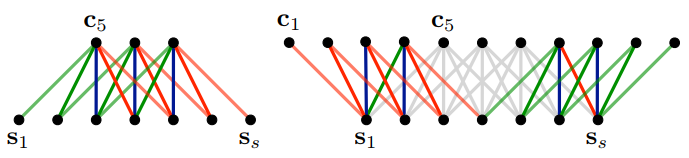
\includegraphics[scale=0.7]{convolution.png}
        \caption{Narrow and wide types of convolution}
        \label{fig:Figure 1}
    \end{figure}
    \item Instead of using max pool they use dynamic $k$-max pooling operation. This returns a sub-sequence of $k$ maximum values in the sequence, instead of a single maximum value. Max pooling operation cannot distinguish whether a relevant feature occurs once or multiple times and it forgets the order in which the features occur. Moreover the pooling factor can be too excessive. The $k$-max pooling operation mitigates these problems. $k$ can be also be a function of length of sentence and the depth of the network. The value of $k$ can be seen as a model of number of values needed to describe a feature of corresponding order. For example first order features such as positive words occur at most $k-1$ times in the sentence, second order features such as negated phrase or clause occur at most $k_2$ times etc.  
    \item Filters in first layer can learn to recognize specific $n$-grams with size less than or equal to the filter size $m$. Filters in the higher layers can capture syntactic or semantic relations between non-continuous phrases that are far apart in the input sentence.  
    \item The dynamic $k$-max pooling operation combined with wide convolution performs better than max pool time delayed convolutional neural network across variety of tasks.

\end{itemize}

\end{document}
